% This is samplepaper.tex, a sample chapter demonstrating the
% LLNCS macro package for Springer Computer Science proceedings;
% Version 2.20 of 2017/10/04
%
\documentclass[runningheads]{llncs}
%
\usepackage{graphicx}
% Used for displaying a sample figure. If possible, figure files should
% be included in EPS format.
%
% If you use the hyperref package, please uncomment the following line
% to display URLs in blue roman font according to Springer's eBook style:
% \renewcommand\UrlFont{\color{blue}\rmfamily}

\begin{document}
%
\title{An awesome visualization of an interesting\\data set with clever methods}
%
%\titlerunning{Abbreviated paper title}
% If the paper title is too long for the running head, you can set
% an abbreviated paper title here
%
\author{First Author \and
Second Author \and
Third Author (alphabetically by last name)}
%
\authorrunning{}
% First names are abbreviated in the running head.
% If there are more than two authors, 'et al.' is used.
%
\institute{TU Wien, Vienna, Austria} %\\
%\email{\{e11111111,e22222222,e33333333\}@student.tuwien.ac.at}}
%
\maketitle              % typeset the header of the contribution
%
%
%
%
%%\section{First Section}

This is a brief description of our visualization of the awesome data set, including some justification for the chosen methods and design choices, pointers to the highlights we are really proud of and maybe some caveats which should be taken into consideration. 

We used the following design rules when creating our submission:
\begin{itemize}
	\item edges are curves
	\item vertices are dots
\end{itemize}

As an example of references and citations if needed: Figure~\ref{fig1} shows the Utah teapot~\cite{blinn1976texture}.

\begin{figure}
	\centering
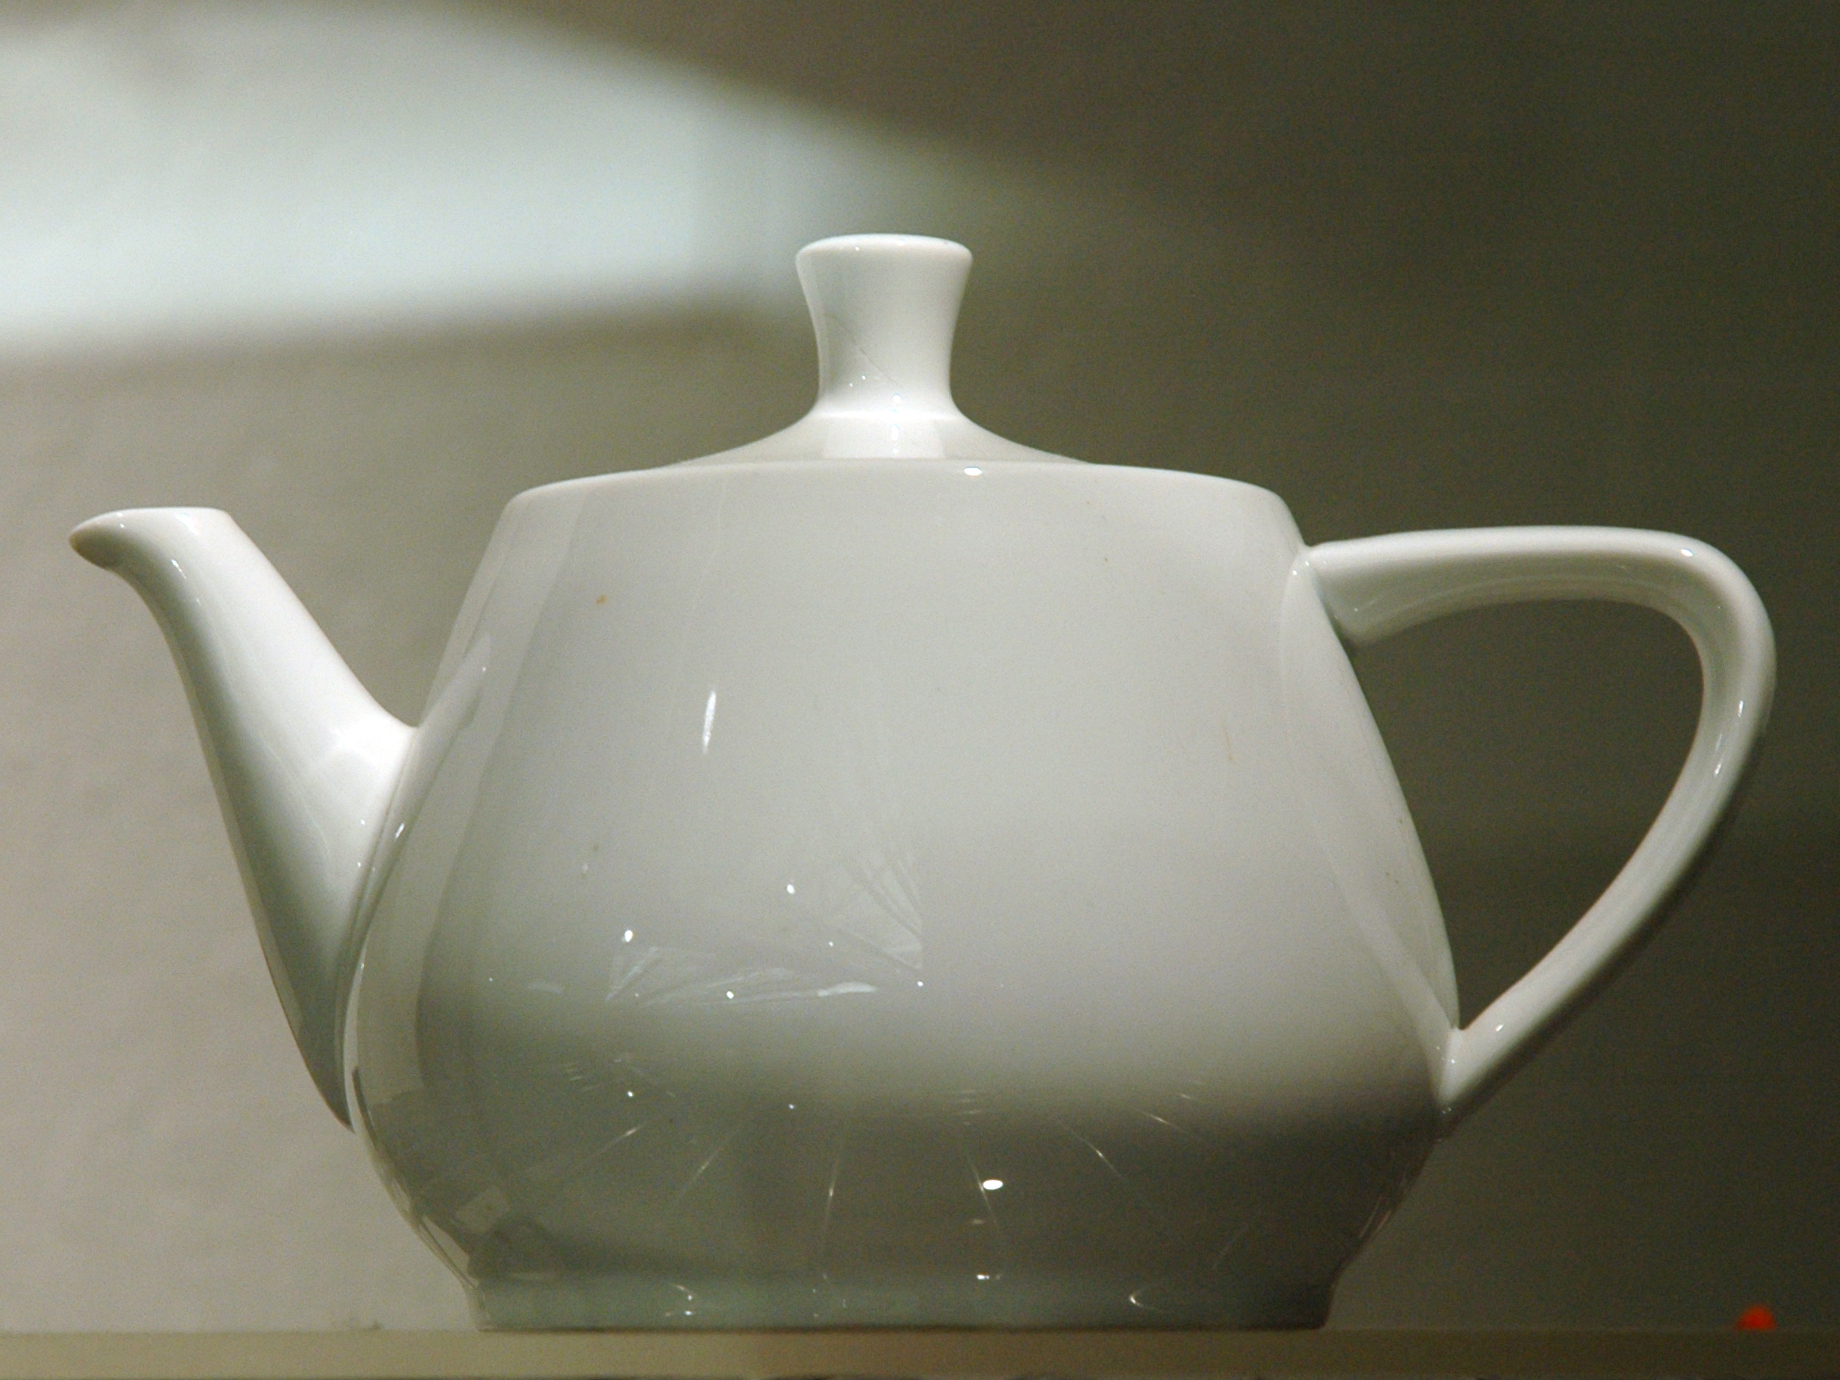
\includegraphics[width=.5\textwidth]{Original_Utah_Teapot.jpg}
\caption{This is how images can be included} \label{fig1}
\end{figure}


The actual contest contribution should be inserted in a PDF merge tool as the second page. (Not via the \LaTeX\ includegraphics command as that would create an ugly white margin around it.)


%
% ---- Bibliography ----
%
% BibTeX users should specify bibliography style 'splncs04'.
% References will then be sorted and formatted in the correct style.
%
 \bibliographystyle{abbrv}
 \bibliography{references}
%
%\begin{thebibliography}{8}
%
%\end{thebibliography}
\end{document}
